\section{User Study: Trust Evaluation}
In the previous section, we discussed three systems with different accuracy levels and three types of explanations. Similar to the experiment discussed in \cite{langer1978mindlessness}, we have built a system offering (1) no explanation for its decision, (2) a placebic explanation (non-informative) for its decision, and (3) an informative (i.e. truthful) information for its decision. In this section we present the user study in which we investigated the influence of model accuracy and explanation fidelity on user trust. We use two approaches to measure user trust: an explicit measure based on a questionnaire and a proxy that measures trust via the willingness to accept and adapt to the system's recommendations.


\subsection{Method}

\paragraph{Participants}
In total, 327 participants took part in the main user study with an average age of 29.4 years (SD = 8.8), a gender balance of 56\% (males) to 43\% (females) and two participants reporting the third gender. 87\% of the participants were recruited via the paid science crowdsourcing platform ``Prolific"\footnote{https://prolific.ac}, while 36 participants enlisted on ``SurveyCircle"\footnote{https://www.surveycircle.com}, an unpaid participant recruitment platform based on mutuality.\newline
On both platforms, individuals younger than 18 years were excluded to participate for reasons of consent by a major. The use case scenario included reading and understanding real-life Tweets with slang words, grammatical and literal errors. The platforms therefore screened for people being fluent in English. 57\% self-assessed their level of English to be equivalent to a native speaker, 23\% as advanced (C1 on the Common European Framework of Reference for Language scale \cite{council2001common}), 14\% as upper-intermediate (B2), and 5\% as lower than that. All participants claimed to be ``fluent" in English. The study questionnaire included an attention check question, asking the participants to answer ``completely disagree" in between the trust questionnaire items assessed on a 5-point Likert scale. Data from participants who failed to answer the attention check correctly was excluded from the analysis. Furthermore, only complete responses were used in the analysis, i.e. data from participants who reached the last page of the survey. The exclusion criteria invalidated 41 data points, resulting in 286 valid cases.\newline
All participants recruited on the paid platform ``Prolific" received a compensation of 1.40 GBP (1.60 EUR) for an estimated completion time of 12 minutes. Participants from ``SurveyCircle" received a reward of 4.4 Study Points.

\paragraph{Apparatus}
The user study was set up as an online study, the study could therefore be taken at a self-chosen location on private devices. Participants were asked to completed the survey on a notebook, desktop computer or tablet. For consistency with the use case scenario, screenshots of a fictive social media management platform showed the input texts, decisions and explanations. The screenshots had a ratio of 900px (width) to 253px (height). To ensure that improper scaling of the screenshots did not influence the participants' perception, devices with small screens (e.g. smartphones and other mobile devices) were excluded. However, which device participants finally used could not be verified. No further requirements were made regarding the equipment of the participant's device.

\paragraph{Procedure}
On both platforms, the participants receive a link to the survey. As soon as the participant has opened the survey URL, the survey starts. The survey consists of the following content:
\begin{enumerate}
	\item Introduction \& consent form
	\item \textit{Scenario 1}: Social media administrator and manual offensive language detection
	\item \textit{Tweet block 1}: 15 Tweets for classification, on individual pages (no system)
	\item \textit{Scenario 2}: Introduction to automatic decision system supporting the task
	\item \textit{Tweet block 2}: Repetition of 15 Tweets for classification, on individual pages (with system)
	\item Perceived understanding \& trust questionnaire
	\item Demographics
	\item Outroduction \& crowdsourcing completion codes
\end{enumerate}
In general, the study contains three blocks plus an introduction and outroduction section. The first block treats a scenario in which the participant plays the role of a ``social media administrator" of a company with a young target group (15-20 years old). The task of the social media administrator is to identify content with offensive language in order to block such comments or Tweets. The next 15 pages of the survey contain one Tweet each, shown on a screenshot of a management tool, and ask the participant to classify the text as offensive or not offensive as shown in figure \ref{fig:survey_tools1}. The order in which the Tweets are shown is randomised for each participant. There are 10 different sets of Tweets available (without overlap), to avoid effects from the specific wording or topics in the small set of 15 Tweets. At the start of the survey, each participant is randomly assigned to one Tweet set by the system.\newline
\begin{figure} [H]
	\centering
	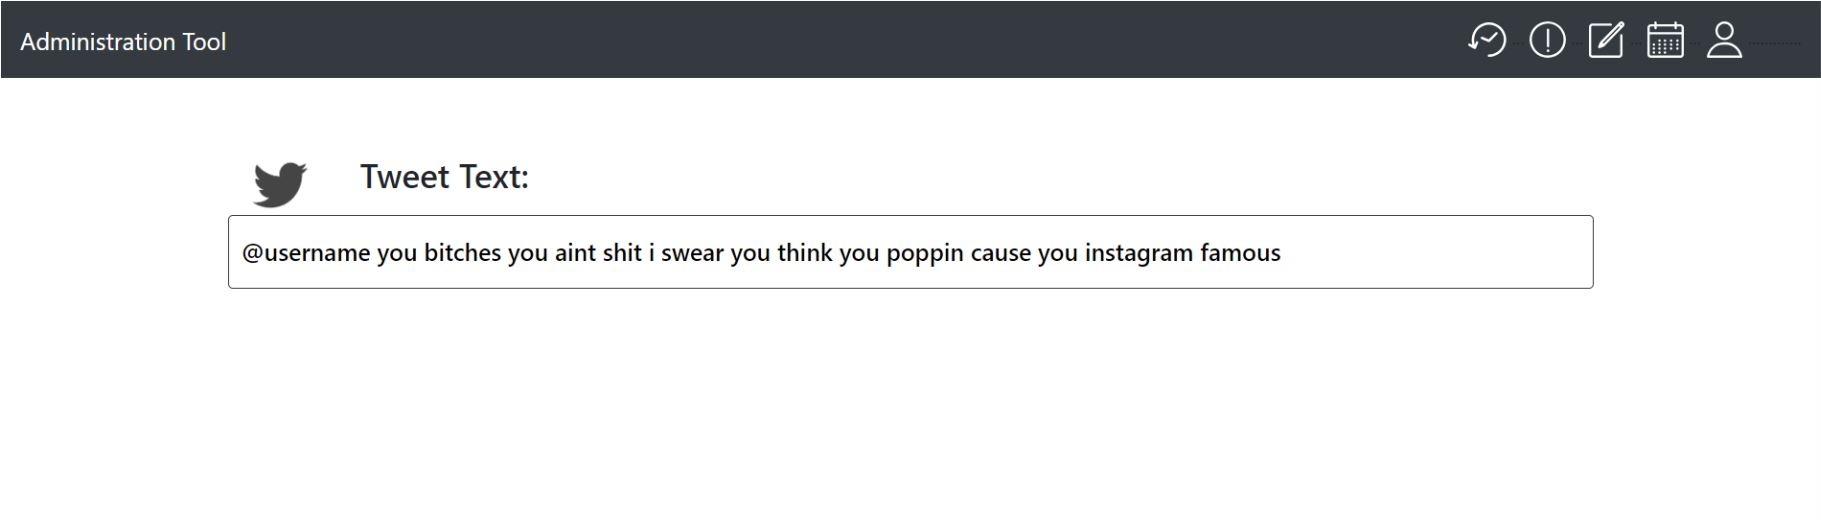
\includegraphics[width=0.8\textwidth]{img/neu_5_13.JPG}\\
	\caption{Screenshot of the fictive management tool without the automatic decision system}
	\label{fig:survey_tools1}
\end{figure}
The second block introduces the automatic decision system (see figure \ref{fig:survey_tools2}). The participant is again asked to classify 15 ``very similar" Tweets, which are, in fact, identical to the ones shown in the first block. This particular formulation aims to liberate the participants from the urge to classify each text with exactly the same label as in the first block. The ordering of the Tweets is random and hence very likely to be different from the ordering of the first block. In total, 9 conditions exist: three systems (classifier with 0.95, 0.75, and 0.05 accuracy) with three explanation types (informative, placebic, no explanation) each. Each participant has one condition assigned at the beginning of the survey, such that there is an equal distribution of conditions in finished questionnaires. \newline
\begin{figure} [H]
	\centering
	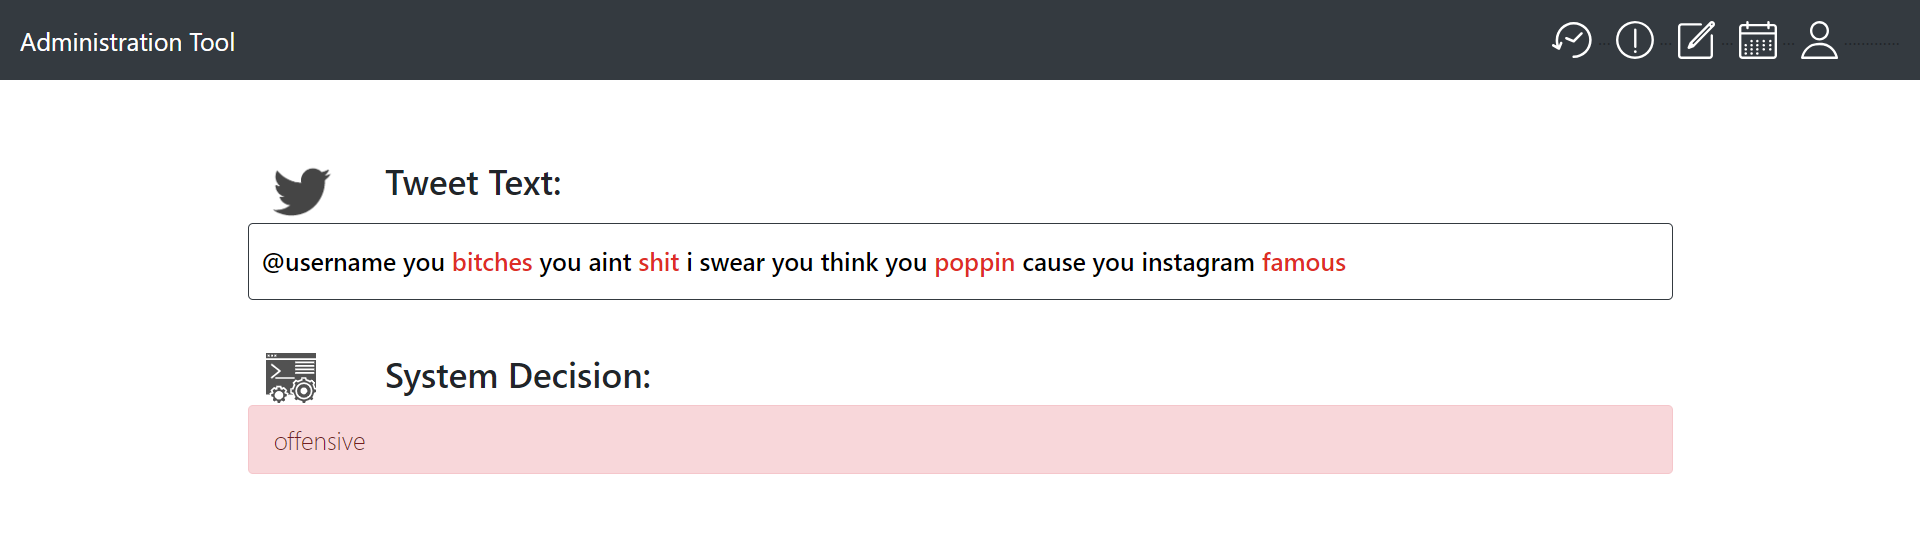
\includegraphics[width=0.8\textwidth]{img/pg_5_13.PNG}
	\caption{Screenshot of the fictive management tool with the automatic decision system}
	\label{fig:survey_tools2}
\end{figure}
Finally, the last block contains three questions regarding perceived understanding, 19 items measuring the user's trust including an attention check, and 5 demographic questions (gender, age, country, ethnicity, English language level).\newline
A detailed list of all questions used in the survey can be found in appendix {\color{red}X}.

\paragraph{Design \& Analysis}
The between-subject setup described in the previous paragraph was tested in a pilot study with 11 participants. The participants were recruited via ``Prolific" and received a compensation of 2.00 GBP (2.28 EUR). They completed the study in ``pretest" mode, which shows an additional comment box at the bottom of each survey page.\newline
The main study was set up as a quantitative study without open questions or free text input. Basic frequency analysis was used for the demographic items in order to understand the background of the participants. Three topics were investigated in a statistical manner: perceived understanding (3 items), self-reported trust (19 items), and observed trust via proxy. For the first two, a 5-point Likert scale was employed.\newline
A \textit{Perceived understanding} score was calculated for each participant by taking the mean of the ratings for all three items in the questionnaire. The trust questionnaire used to measure \textit{self-reported trust} contains 14 positive items and 5 inverse items. A single mean score was calculated by taking the average over the positive items and the maximum rating minus the mean of the inverse items. As a second trust measure, \textit{observed trust} was investigated via the proxy of willingness to follow a system's recommendation. The survey contained one block of manual classification without the system, and a second round with the information provided by the automated decision system. In each block, participants classified the same set of Tweets. We can therefore determine how often a participant switched his or her classification out of 15 possible cases and how often the change was made in agreement with the classifier's prediction but against the truth. Since the three classifiers offered different amount of opportunities to change with the classifier's prediction away from the truth (maximum 14 cases for the bad classifier as opposed to maximum 1 case for the very good classifier), the proxy measure is calculated and normalised as follows for each participant:
\[ \frac{changes\_towards\_prediction\_against\_truth}{opportunities\_for\_change\_against\_truth} \]
Cases in which the very good classifier did not make any misclassification (hence no opportunity for the user to change in favour of the classifier and in contradiction to the truth) were excluded, because no valid conclusion can be drawn from these cases. 42 cases occurring in the conditions with the very good classifier had to be excluded due to this issue.\newline
%14,17,23 = 54
%30,32,34 = 96 
%96-54 = 42
The goal of the statistical analysis for all three topics (perceived understanding, self-reported trust, observed trust via proxy) is to identify differences between different conditions. Not all samples were normally distributed, which we investigated with the Shapiro-Wilk test \footnote{https://docs.scipy.org/doc/scipy/reference/generated/scipy.stats.shapiro.html} for normality from the SciPy library). We therefore used the Mann-Whitney U test to compare two samples, since it does not assume normal distribution nor equal sample sizes or variances. For sample sizes above 20 data points, we employed SciPy's approximation\footnote{https://docs.scipy.org/doc/scipy/reference/generated/scipy.stats.mannwhitneyu.html} of the Mann-Whitney U test. For smaller sample sizes - only occurring in the observed trust via proxy scores where data points had to be excluded -, we used the exact implementation\footnote{https://mail.python.org/pipermail/scipy-dev/2015-March/020475.html} of the Mann-Whitney U test as described in \cite{cheung1997mann}.


\subsection{Results}
The following section presents the results of the user study. We examined perceived understanding, self-reported trust and an implicit trust measure via the willingness to follow a classifier's recommendation. For each topic, we give the mean score, standard deviation, as well as a comparison of all conditions in a 9x9 matrix.\newline
The matrices show each condition checked for significant difference with every other condition. The colour scale is a visualisation of the p-value: Insignificant p-values, i.e. values above the critical threshold of 0.05, are coloured in dark blue, while significant p-values are presented with colours from blue over green to light yellow. P-values marked as ``0" are too small (below 0.001) to be displayed correctly in the matrix.\newline 

\paragraph{Perceived Understanding}
As figure \ref{fig:results_understanding} shows, users of the system with a very good classifier and no explanation report the highest perceived understanding. For the very good and the medium classifier, giving no explanations for the decisions leads to a higher perceived understanding than delivering placebic, i.e. random, explanations. In general, users have more confidence in their understanding of the system for the very good and medium classifiers as compared to the bad classifier. One condition, however, does not lead to significantly higher scores than the bad classifier: for the medium classifier with random explanations, users reported the same understanding as for the bad classifier with no explanations. Concerning the bad classifier, giving a truthful explanation for the decision leads to the lowest perceived understanding.
\begin{figure}[H]
	\begin{subfigure}[b]{0.3\textwidth}
		\raisebox{80pt}{\resizebox{\textwidth}{!}{
				\begin{tabular}{lrr}
					\textbf{Condition} & \textbf{Mean} & \textbf{SD} \\ \midrule
					super-good & 11.833 & 2.746 \\
					super-rand & 11.188 & 2.579 \\
					super-no & 12.441 & 2.103 \\
					medium-good & 11.455 & 2.475 \\
					medium-rand & 8.833 & 2.888 \\
					medium-no & 11.100 & 2.071 \\
					bad-good & 7.395 & 3.602 \\
					bad-rand & 7.500 & 3.413 \\
					bad-no & 8.833 & 3.455 \\ \bottomrule
		\end{tabular}}}
		\caption{Mean and standard deviation per condition}
		\label{tab:results_table_understanding}
	\end{subfigure}
	\begin{subfigure}[b]{0.65\textwidth}
		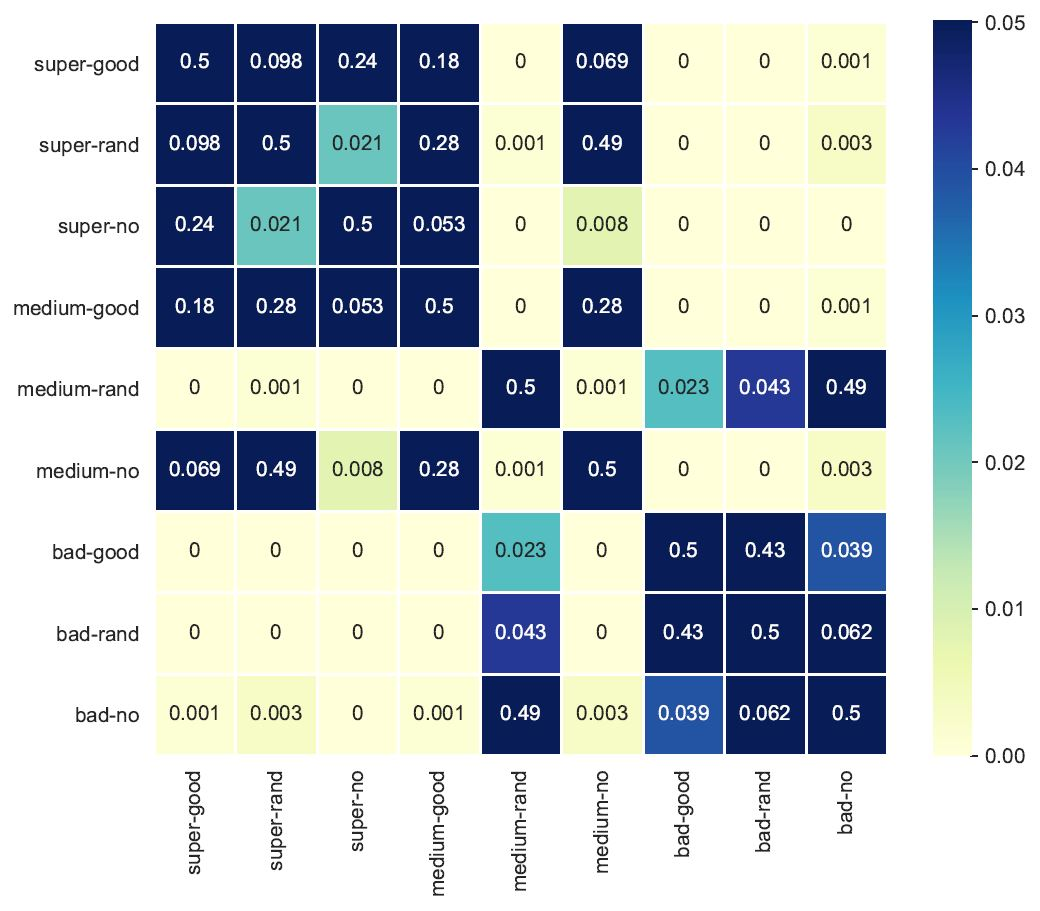
\includegraphics[width=\textwidth]{img/results_matrix_understanding2.JPG}
		\caption{Significance matrix with p-values per condition}
		\label{fig:results_matrix_understanding}
	\end{subfigure}
	\caption{Results for perceived understanding scores}
	\label{fig:results_understanding}
\end{figure}


\paragraph{Trust Questionnaire}
The self-reported trust scores show similar results as the perceived understanding: Besides the medium classifier with random explanations, all systems lead to significantly more trust than the systems employing the bad classifier. The explanations do not play a role regarding user's trust when the bad classifier is used. Looking at the medium classifier, the random explanation leads to a lower trust score than no explanation and a good explanation, with no difference between the latter two. The most trust is evoked by the very good classifier without explanations, significantly more than for any other condition. There is no significant difference between the very good classifier with explanations and the medium classifier with meaningful explanation. For both the bad classifier and the very good classifier, the condition without any explanation again led to the highest scores within the same classifiers. The detailed results are presented in figure \ref{fig:results_trust}.
\begin{figure}[H]
	\begin{subfigure}[b]{0.3\textwidth}
		 \raisebox{80pt}{\resizebox{\textwidth}{!}{
		\begin{tabular}{lrr}
			\textbf{Condition} & \textbf{Mean} & \textbf{SD} \\ \midrule
			super-good & 50.967 & 7.600 \\
			super-rand & 50.906 & 9.156 \\
			super-no & 56.912 & 9.721 \\
			medium-good & 50.030 & 9.150 \\
			medium-rand & 42.000 & 9.671 \\
			medium-no & 49.967 & 8.712 \\
			bad-good & 36.421 & 8.129 \\
			bad-rand & 37.067 & 7.659 \\
			bad-no & 38.333 & 10.381 \\ \bottomrule
		\end{tabular}}}
		\caption{Mean and standard deviation per condition}
		\label{tab:results_table_trust}
	\end{subfigure}
	\begin{subfigure}[b]{0.65\textwidth}
		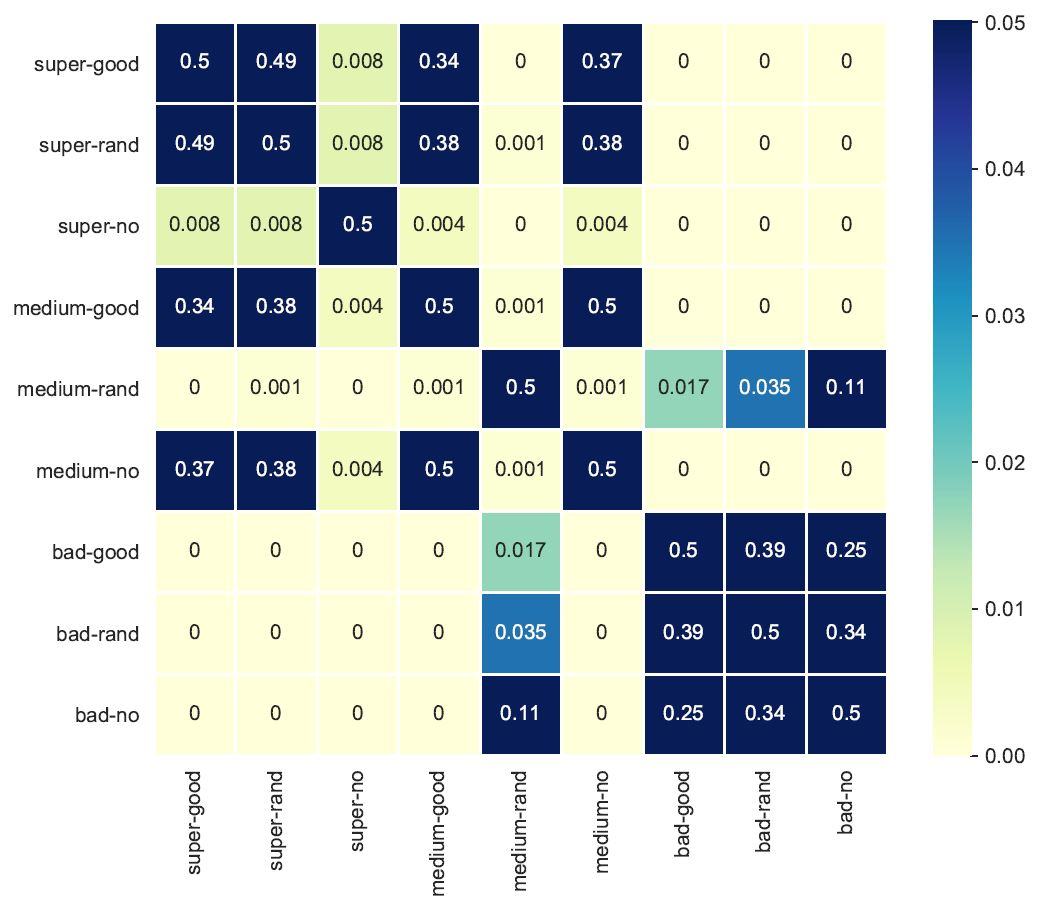
\includegraphics[width=\textwidth]{img/results_matrix_trust2.JPG}
		\caption{Significance matrix with p-values per condition}
		\label{fig:results_matrix_trust}
	\end{subfigure}
	\caption{Results for self-reported trust scores}
	\label{fig:results_trust}
\end{figure}



\paragraph{Observed Trust via Proxy}
The second trust measure uses a proxy to determine the trust a user puts into a system: the willingness to follow a system's recommendation, in this case the decision about offensiveness and non-offensiveness. Figure \ref{fig:results_proxy_away} shows the results of analysing the user's willingness to change a classification to match the system's decision while contradicting the truth. As a comparison, figure \ref{fig:results_proxy_towards} deals with changes in classification that were made in favour of both the system and the truth.\newline
The results presented in this section need to be analysed with caution. Consider the case of the very good classifier with meaningful explanations. Out of 30 cases in this condition, 16 did not have the possibility to show a change away from the truth towards the prediction of the classifier, because the classifier in those 16 cases did not make any mistakes. From the remaining 14 cases, 4 showed the behaviour in question, leading to a mean of 0.286. This result is rather high, compared to the other conditions' mean scores. The same issue appears in the data for changing from a faulty classification towards a correct classification in accordance with the bad classifier: Each participant in this condition had at maximum once the possibility to show the behaviour in question. Seen that the number of participants in each group is not large to begin with, which is then reduced by the number of cases where such behaviour is not possible, the remaining sample size is very small for solid statistical analysis.\newline
The highest changing rate in favour of the system but against the true label was detected for users of the very good classifier with a meaningful explanation, but also the highest variance. Users were significantly more likely to adapt the system's faulty decision when confronted with the very good system with random and no explanations than the users of any system with the bad classifier. The same holds true for users of the medium classifier without explanations.\newline
\begin{figure}[H]
	\begin{subfigure}[b]{0.3\textwidth}
		\raisebox{80pt}{\resizebox{\textwidth}{!}{
				\begin{tabular}{lrr}
					\textbf{Condition} & \textbf{Mean} & \textbf{SD} \\ \midrule
					super-good & 0.286 & 0.452 \\
					super-rand & 0.118 & 0.322 \\
					super-no & 0.043 & 0.204 \\
					medium-good & 0.088 & 0.189 \\
					medium-rand & 0.083 & 0.158 \\
					medium-no & 0.075 & 0.183 \\
					bad-good & 0.050 & 0.066 \\
					bad-rand & 0.054 & 0.067 \\
					bad-no & 0.073 & 0.093 \\ \bottomrule
		\end{tabular}}}
		\caption{Mean and standard deviation per condition}
		\label{tab:results_table_proxy_away}
	\end{subfigure}
	\begin{subfigure}[b]{0.65\textwidth}
		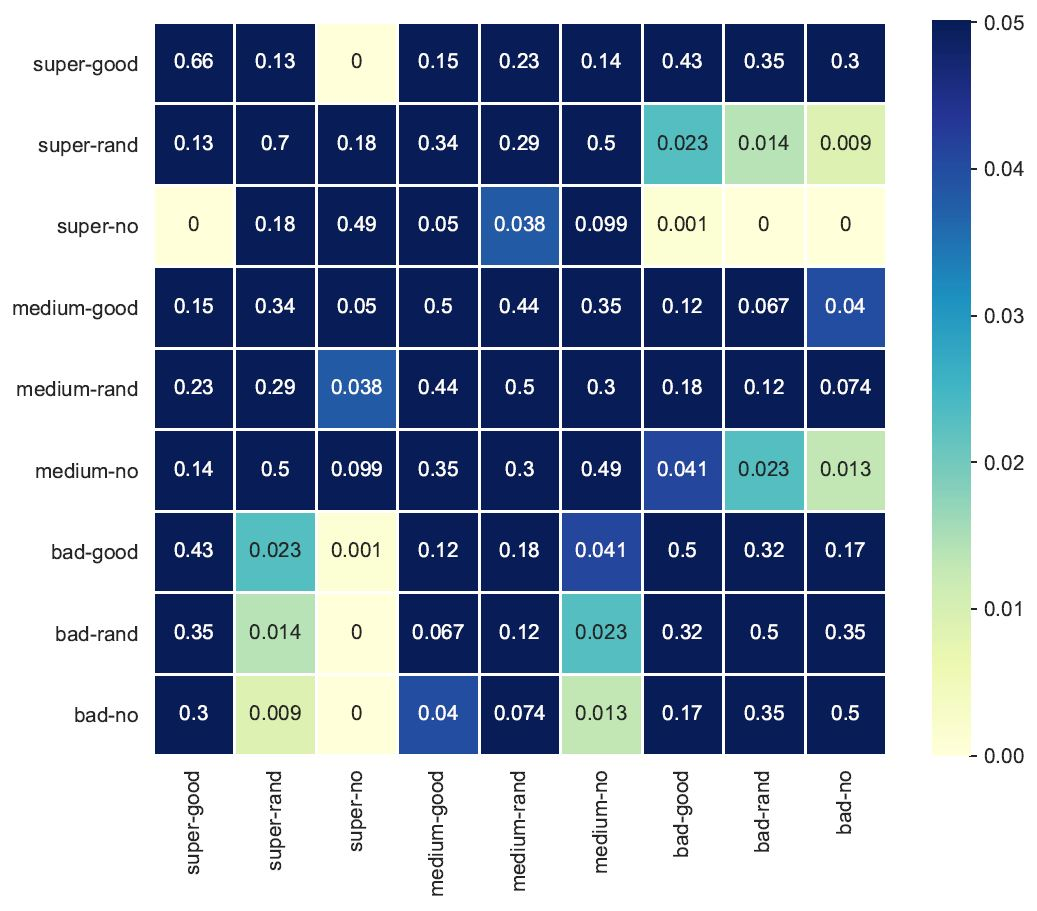
\includegraphics[width=\textwidth]{img/results_matrix_proxy_away2.JPG}
		\caption{Significance matrix with p-values per condition}
		\label{fig:results_matrix_proxy_away}
	\end{subfigure}
	\caption{Results for proxy measure of trust via willingness to accept the system's prediction changing manual label away from actual truth}
	\label{fig:results_proxy_away}
\end{figure}
Looking at the changes made towards the truth in agreement with the classifiers, no significant differences are noted between any condition with the very good and medium classifier. The same holds true for the bad classifier. The very good and medium classifiers, however, evoked significantly more changes towards the truth than the bad classifier with explanations. The standard deviations of the conditions using the bad classifier are rather high as compared to any other condition.\newline
One condition is exceptional in this analysis: Although the bad classifier without explanation has the highest mean score (i.e. changes towards the truth when the classifier made a correct prediction), the score is not significantly different from the bad classifier with a good and random explanation. The variance of all three systems (bad-no, bad-random, bad-good) are very high as compared to the variances of the other systems. The score deviates, however, from the results of the very good and medium classifier, which have lower mean scores but lower variances. The difference in variance is important to note when comparing the relatively high mean score of the bad classifier without explanation to the conditions with the very good and medium classifiers.
\begin{figure}[H]
	\begin{subfigure}[b]{0.3\textwidth}
		\raisebox{80pt}{\resizebox{\textwidth}{!}{
				\begin{tabular}{lrr}
					\textbf{Condition} & \textbf{Mean} & \textbf{SD} \\ \midrule
					super-good & 0.073 & 0.073 \\
					super-rand & 0.047 & 0.064 \\
					super-no & 0.063 & 0.093 \\
					medium-good & 0.058 & 0.087 \\
					medium-rand & 0.049 & 0.070 \\
					medium-no & 0.058 & 0.066 \\
					bad-good & 0.048 & 0.213 \\
					bad-rand & 0.045 & 0.208 \\
					bad-no & 0.091 & 0.287 \\ \bottomrule
		\end{tabular}}}
		\caption{Mean and standard deviation per condition}
		\label{tab:results_table_proxy_towards}
	\end{subfigure}
	\begin{subfigure}[b]{0.65\textwidth}
		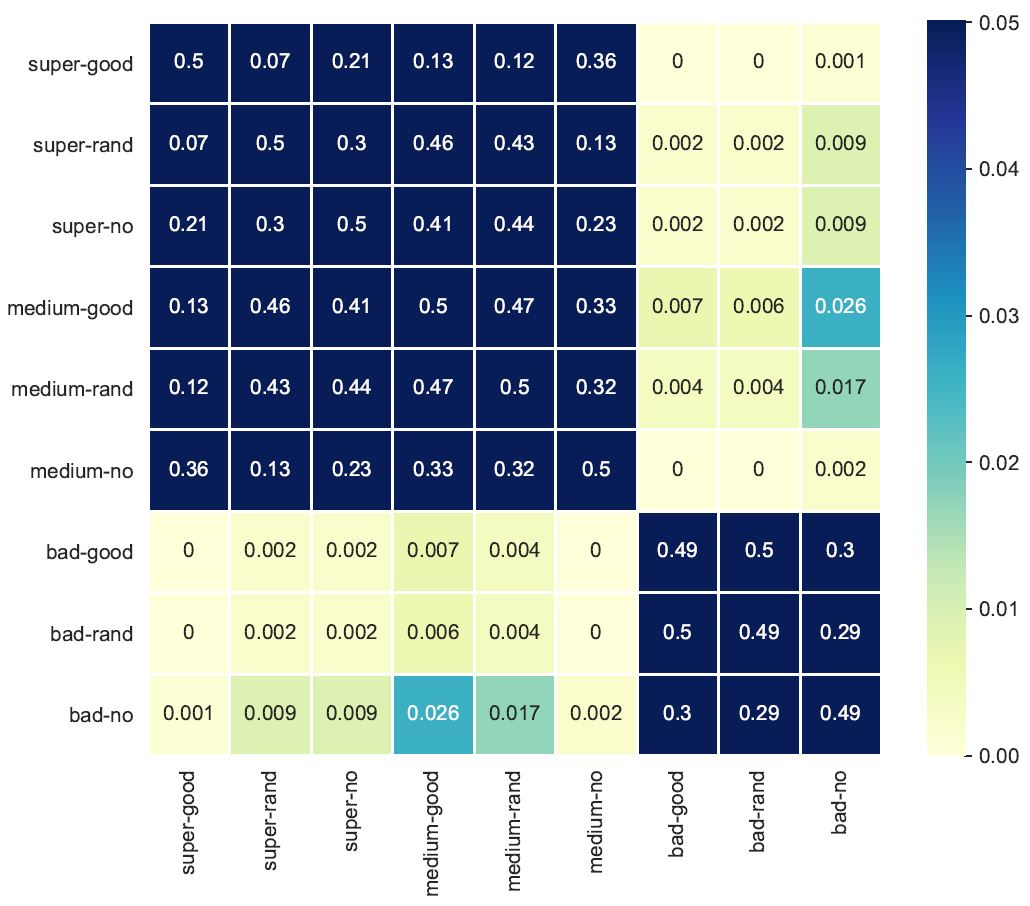
\includegraphics[width=\textwidth]{img/results_matrix_proxy_towards2.JPG}
		\caption{Significance matrix with p-values per condition}
		\label{fig:results_matrix_proxy_towards}
	\end{subfigure}
	\caption{Results for proxy measure of trust via willingness to accept the system's prediction changing the manual label towards the truth}
	\label{fig:results_proxy_towards}
\end{figure}



\subsection{Discussion}
%-------------------------------------------------------------------------
% RQ 1: effect of accuracy on trust
Our results suggest that \textit{both perceived understanding and trust are positively related to the classifier's accuracy in general} (\textbf{RQ 1}). The higher the accuracy, the higher the trust in the system. The strongest evidence is found in the reactions to the classifiers without explanations (super-no, medium-no, bad-no). The self-reported trust was the highest for the best classifier and the lowest for the bad classifier, with all scores differing significantly from each other. The same can be observed even when adding the bad explanations: The very good classifier still has significantly higher trust and perceived understanding scores than the other classifiers, with the bad classifier again having the lowest scores. The good explanation, however, influences the trust and perceived understanding differently. Here, the bad classifier still receives significantly worse trust and understanding scores than the other two, yet there is no difference anymore in the scores for the very good and medium classifiers. \newline
An explanation for the similarity of both the trust score and the perceived understanding score for super-good and medium-good could be the persuasiveness of a good explanation. The difference in trust and perceived understanding, that we see between the very good and medium classifier in the condition without explanation, could be compensated by convincing the user of the classifier's trustworthiness through a good explanation.\newline
It seems intuitive to have higher trust in a system that leads to fewer deception, which has also been described in \cite{glass2008toward} with the ``expectation mismatch" (see section \ref{subsubsec:trust_factors}). A classifier with high accuracy effectively leads to fewer disappointed expectations, which in turn does not decrease the trust. Furthermore, the set size of 15 Tweets seems to be enough for users to develop an intuition about the classifier's accuracy. Whether users start with a high trust level and decrease the trust with every mismatch, or have a basic trust level that is increased with expectation matches and decreased with every mismatch remains to be examined in future research. The results also do not deliver information about the proportionality of accuracy and the trust level, which could be a topic of future research as well. \medskip \newline
%-----------------------------------------------------------------------
% RQ 2: effects of explanation types on trust
In the copy machine experiment by \cite{langer1978mindlessness}, only the pure presence of an explanation was enough to make people comply with a request resulting in a short waiting time. On the basis of that experiment, we designed three explanations similar to the setup in \cite{langer1978mindlessness}: No explanation, placebic explanation, and a meaningful explanation for the classifier's behaviour. Similar to the results of the copy machine experiment, we expected to see no difference between trust scores of the meaningful and placebic explanation but a difference between the two explanations and the no explanation settings. The results, however, show a mixed answer.\newline
For the \textit{very good classifier}, the meaningful and placebic explanation indeed led to the same trust score. Other than expected, the no explanation condition showed the best results. The classifier performed at an accuracy of 0.95, which resulted in 44\% of the cases in a perfect classification rate within the small subset of 15 Tweets. A possible explanation for the good trust score in the no explanation condition could be the conservation of a perfect image throughout the 15 Tweets. The classifier makes (almost) no mistakes and does not offer any information that could lead to doubts about the classifier's abilities. Both displayed explanation types would then have a disadvantage over the no explanation condition: The good explanations are not necessarily meaningful to a human, as they are based on statistical information rather than semantics or intentions. The placebic explanation is generated at random, which likewise holds potential for doubts and incomprehension. A similar guess was ventured in \cite{cramer2008effects}, who suspected that more knowledge about system boundaries and unfulfilled preferences leads to a decrease in trust (see section \ref{subsubsec:trust_factors}). The opposite can be observed in the proxy measure for trust, i.e. the changes in labelling that a user made towards the classifier's decision but away from the truth. Here, the no explanation condition led to significantly fewer changes away from the truth as compared to the two conditions giving any type of explanation, which is in turn consistent with the results in the copy machine experiment. It is important to note that the copy machine experiment only worked while people are in a ``mindless" state, i.e. an inattentive state of mind. It is possible that users did not in particular pay attention to their trust towards the system during the classification task, but actively reflected on their relationship with the system during the self-report of trust. Being in a mindless state during the proxy measurement while being mindful during the trust questionnaire would explain the conflicting results of both measures.\newline
The results for the \textit{medium classifier} differ from those of the very good classifier. The two conditions with explanations have significantly different trust scores. The placebic explanation has the lowest score, while the meaningful explanation is ranked at the same trust level as the system without explanation. The classifier delivers faulty classifications in three to four cases out of 15, which presumably raises doubts about the system. The negative effect of placebic explanations could therefore be worsened. The ``expectation mismatch" is then twofold, with the wrong classification on the one side and the useless explanation on the other side. With the good explanations, the users receive some information about the underlying reasons for a misclassification. Even if not all information of the explanation is meaningful to a human, it delivers hints to the system's function and malfunction, possibly raising overall trust.\newline
The \textit{bad classifier} did not show evidence of diverting trust scores for any of the three explanation types. The same homogeneity is found in the results of the proxy measurement of trust, for both the changes away from the truth and towards. The trust scores were significantly lower than any other condition, with one exemption. The bad classifier without explanation had comparable trust ratings as the medium classifier with random explanations. Since there is a significant distance between the scores of the medium classifier with random explanations and other conditions of the medium classifier, we conclude that it is due to a property of the medium-random system rather than a phenomenon of the bad classifier. The evidence suggests that users are not fooled by a bad classifier and do not trust it, no matter the explanation given. A plausible assumption could have been that users trust a bad classifier as it is predictable, but do not use it as a basis for their decisions because it is not accurate. This distinction, however, is not found in the results.\newline
Overall, we found evidence that the accuracy of a classifier is more important for trust than the explanation. The explanations did not make a difference for the very good classifier nor the very bad classifier (\textbf{RQ 2}). The case of the medium classifier is an interesting one, as we found an influence of the explanations on user trust here. It would be interesting to investigate the relationship of users with the medium classifier in more detail in future research. The findings also show that an evaluation of explanations in xAI should not only be made for extreme cases, but also consider the - supposedly more realistic - cases on the whole spectrum between the extremes. \medskip \newline
%--------------------------------------------------------------------------------
% RQ 3: effect of explanation types on perceived understanding
One of the factors contributing to trust is \textit{perceived understanding}. Our findings show a negative influence of meaningless information on perceived understanding (\textbf{RQ 3}). For both the medium classifier and the very good classifier, perceived understanding was the worst when delivering placebic explanations. Although actual understanding is arguably different when comparing a case without any explanation and one with good, meaningful information, the perception of knowledge about both cases is equal here. A mechanism similar to ``expectation mismatch" could be in place for perception of knowledge. While building the mental model of the classifiers, no conflicting information have to be consolidated for the good explanation and the no explanation cases. Being confronted with random and therefore meaningless explanations forces the user to unite conflicting information in the mental model. The more conflicts appear, the lower the confidence in the mental model.\newline
For the bad classifier, perceived understanding ratings are significantly lower as for other classifiers (except for medium-random, which has a low rating as well). However, the system delivering good explanations for the faulty behaviour receives a significantly higher score than no explanation and placebic explanation cases. The positive effect of high accuracy does not hold here because the classifier performs badly on the task. Yet, as the explanations give more information about the inner workings of the classifier, it seems intuitive to evoke more confidence of understanding in this case. \medskip \newline
%--------------------------------------------------------------------------------
% Further discussions
In this research, we used a computational evaluation to validate the fidelity of the automatically generated explanations. Although the ``meaningful" explanations demonstrably represent the features that are decisive for the classification, they are not necessarily meaningful to a human observer. We showed in section \ref{subsec:expleval} that the selected words in the texts were enough to reconstruct the behaviour of the classifiers and can therefore serve as a basis for decision. Whether the selection of words is enough for humans to judge is up to discussion. Further research is necessary to determine the actual ``meaningfulness" of the generated explanations for humans.\newline
The proxy measurement of trust via changes in classification between the first and second block of Tweets showed ambiguous results with high variance. For future projects dealing with trust in computer systems, it could be useful to measure trust not only via a questionnaire that requires reflection abilities and active processing of the relationship between user and system. Using a trust measure that can be determined without the participant knowing could serve as an additional view on the practical implications of trust.